\section{Examples}
\subsection{A simple case}
The first example we are going to report is very simple but quite instructive.
We simulated a data sample cointaining two classes of event with Gaussian
signal distributions with different mean values and same width.

In Fig.~\ref{fig:Gaus2} the simulated detector responses and the amplitudes
functions derived in such a case a reported. As it can be noted the amplitudes
$\psi_{i}$ are constructed in order to garantee orthogonality with the $p_{k}$
functions for $i \neq k$.

\begin{figure}[!htb]
\centering
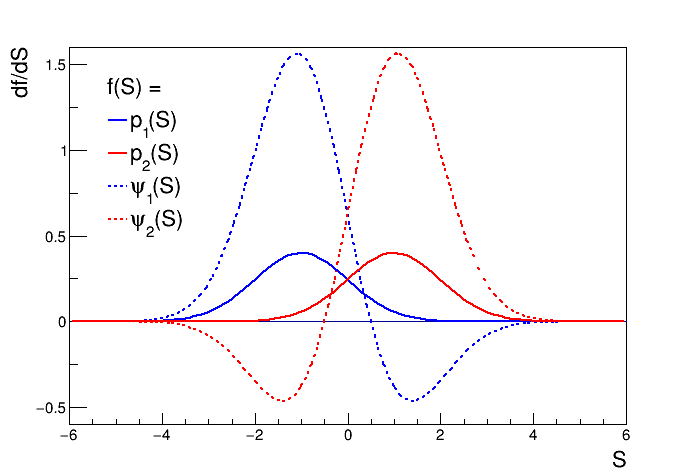
\includegraphics[width=0.7\textwidth]{../png/figGaus2.png}
\caption{Two Gaussian detector responses ($\Delta_{12} = 2$) and relative
  $\psi(S)$ amplitudes.}
\label{fig:Gaus2}
\end{figure}

This is much clearly visible in Fig.~\ref{fig:SPGaus2} where the 4 products
are shown.

\begin{figure}[!htb]
\centering
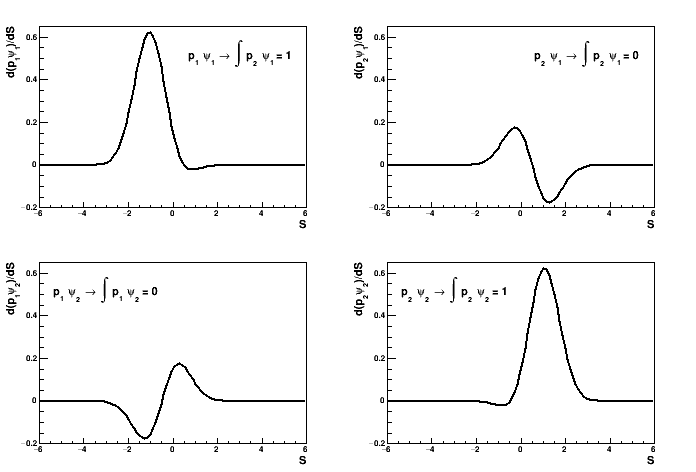
\includegraphics[width=0.7\textwidth]{../png/figSPgaus.png}
\caption{Scalar product functions for the two Gaussian responses case ($\Delta_{12} = 2$).}
\label{fig:SPGaus2}
\end{figure}

To verify the effectiveness of the methods we simulated a sample of $10^5$
events distributed on the two classes with relative abundances of 70\% and
30\% respectively.
Therefore, the event signals generated are distributed as shown in
Fig.~\ref{fig:InputGaus2} where a double Gaussian structure is reported.

\begin{figure}[!htb]
\centering
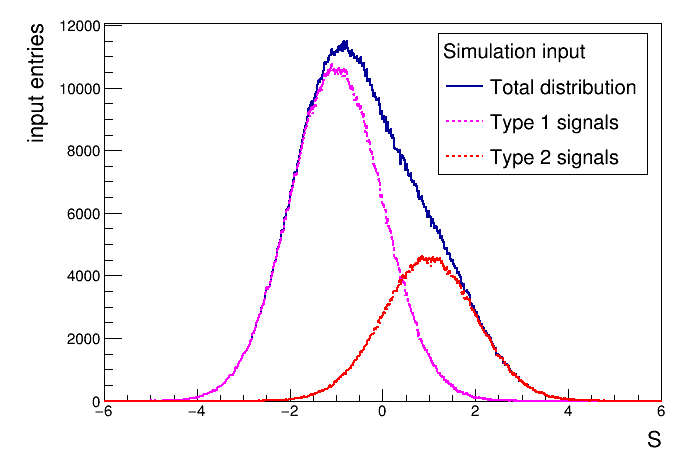
\includegraphics[width=0.7\textwidth]{../png/figInput.png}
\caption{Inputs of the simulation with $\Delta_{12} = 2$ (type 1: 70\%, type 2: 30\%).}
\label{fig:InputGaus2}
\end{figure}

In order to validate the methods the signals generated were processed/counted
for all the events and weighted with the Bayesian probability or
alternativelly with the QM amplitude.
For the Bayesian approach the procedure was iterated in 20 steps with
different set of prior probability. To avoid any bias we started assuming
equal abundances at step 1 and the ones obtained from the previous step
($n-1$) for the n-th step.

In Fig.~\ref{fig:IterGaus2} the results obtained with the two methods are
reported for the case presented and for a similar simulation with a worse
separation between the two classes $\Delta_{12} = 1$.
As it can be noted, while the QM approach returns the correct result at the
first step, the Bayesian appraoch needs more step to reach a convergence to
the truth. The speed of the convergence is high in the first case
($\Delta_{12} = 2$) when a good separation is assumed, while it is quite slow
when the separation is at the level of $1\sigma$.

\begin{figure}[!htb]
\centering
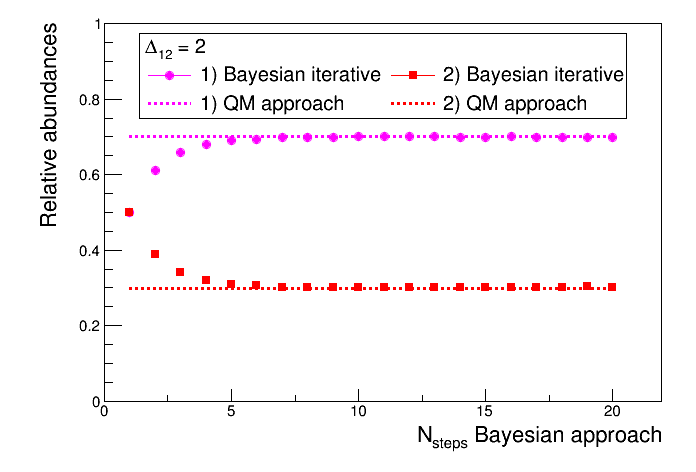
\includegraphics[width=0.45\textwidth]{../png/figIterativeDelta2.png}
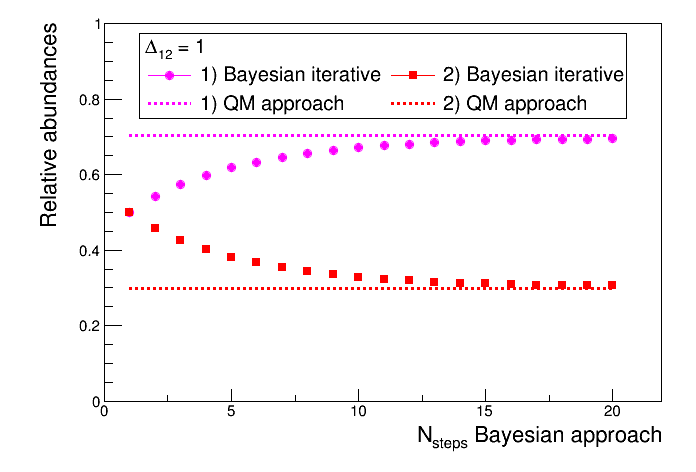
\includegraphics[width=0.45\textwidth]{../png/figIterativeDelta1.png}
\caption{Comparison of the two approaches: results for $\Delta_{12} = 2$ and
  $\Delta_{12} = 1$ cases.}
\label{fig:IterGaus2}
\end{figure}

In any case the two methods are consistent as expected.

\subsection{Multi-variables case}

\subsection{Correlations of event pair}

\newpage
